\chapter{Evaluation}

The following chapter describes the evaulation and introduces the results from the testing of the prototype. 

\section{Purpose of Evaluation}

The following evaluation has been conducted to test the system. The system has been tested internally to test whether the system is stable or not. 
A user test has been conducted to test if the user are able to use the system and evaulate their opinion of the system. 


\section{Internal Test}

To test the accuracy of the prototype, an internal test were carried out. The following hypotheses has been stated for the internal test: \\\\
H\textsubscript{0}: The system works 95\% of the time.\\
H\textsubscript{A}: The system does not work 95\% of the time.\\\\

The test consisted of the copper plates being connected 25 times each. Firstly the index finger were tested with the thumb, secondly the middle finger. Whenever the yellow light on the system
lit up, it was considered a success. If the light did not turn on, it was considered a failure. The times it succeeded and failed were counted.\\\\

The results ended up being as follows:\\
Index finger connection test: 23 out of 25. \\
Middle finger connection test: 25 out of 25.\\\\


The results has been analysed statistically using R\citep{R}. R is a language used for statistical analysis. All the statistics has been calculated with a probability of succes at 95\%.\\\\
The results from the index finger connection test showed a p-value of 0.3576 which is less than the significance level of 0.5. 
Whenever the p-value is less than 0.5 the H\textsubscript{0} is rejected. Which means that the system did not work 95\% of the time. \\

The results for the middle finger connection test, showed a p-value of 0.635 which means that the H\textsubscript{0} is accepted,
and that connection works at least 95\% of the time. \\

Another internal test has been carried out to test the accuracy of the effects. The test were conducted in a similar way, the effect were applied and then used. 
As long as the effect worked and changed the voice input, it was considered a success. \\\\
The system worked 18 out of 25 times. \\\\

Since the gesture effects showed the same results, the p-value is the same for both gestures. 
The p-value ended up being 0.00016 which is lower than 0.5 and therefore the H\textsubscript{0} is rejected. 
Meaning that the gestures did not work 95\% of the time. \\

During the first tests, the system had a loose wire. The issue were fixed and the tests were then conducted once again. With the following results:\\\\
All the tests worked 25 out of 25 times. \\
This gave a p-value of 0.635 which is more than 0.5 and therefore the H\textsubscript{0} is accepted. 

\section{User Test}

%Intro

\subsection{Evaluation Plan}
When conducting this user test, it is the intention to get some data from the users about the different effects and gestures. 
Initially, the users are asked to sign a consent form, see Appendix \ref{Consent} and \ref{Script} for script and consent form. They are then told to put on the glove and try to apply the effects. Afterwards, they are then asked to answer a questionnaire, see Appendix \ref{Questionnaire}. 

\subsection{Apparatus and Setup}

To perform the test, the following equipment is needed:
\begin{itemize}
 \item Two laptops
 \item Zoom H4N microphone 
 \item Headphones
 \item The Protoype
\end{itemize}

The following figure \ref{Setup} shows the setup of the evaulation. One person wearing the system, a facilitator and one person that makes sure the system works. 

\begin{minipage}{\linewidth}% to keep image and caption on one page
\makebox[\linewidth]{%        to center the image
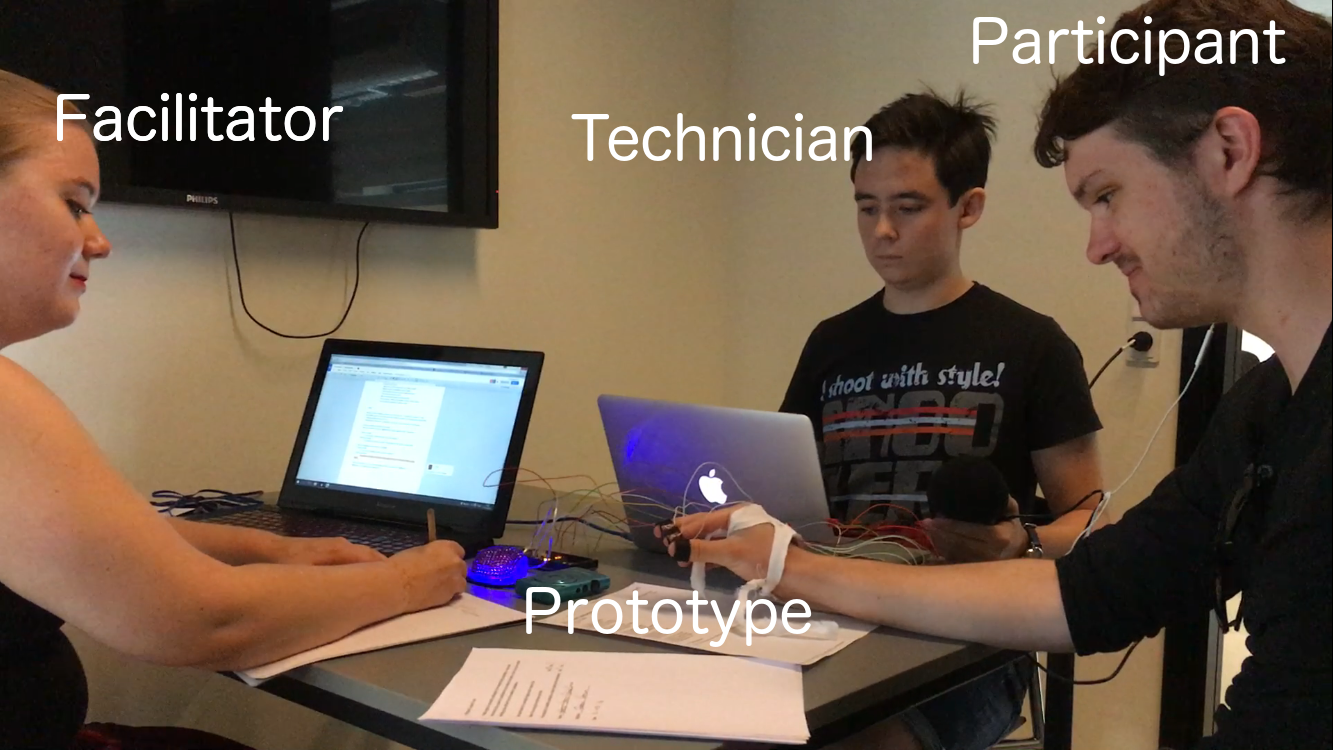
\includegraphics[keepaspectratio=true,scale=0.1]{Setup}}
\captionof{figure}{The Test Setup}\label{Setup}
\end{minipage}\\

\subsection{Results}


\subsection{Analysis}

\subsection{Theory}


\section{Conclusion}